\subsection{矩形}\label{subsec:czjh1-4-5}

根据四边形的不隐定性,我们可以把一个平行四边形的形状改变成有一个直角的平行四边形(图 \ref{fig:czjh1-4-20})。
有一个角是直角的平行四边形叫做\zhongdian{矩形}(通常也叫做\zhongdian{长方形})。
矩形是人们日常生活和生产中最常见的四边形,如课本,黑板、门、窗等都呈矩形。

% \begin{figure}[htbp]
%     \centering
%     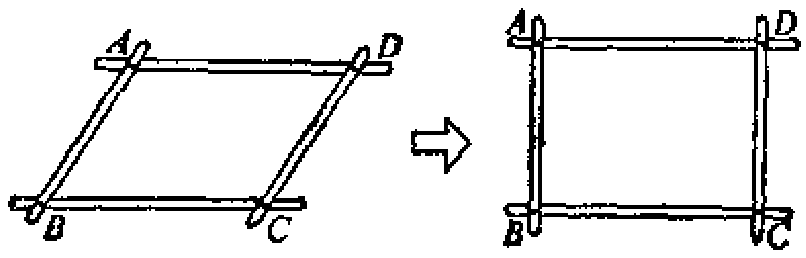
\includegraphics[width=6cm]{../pic/czjh1-ch4-20.png}
%     \caption{}\label{fig:czjh1-4-20}
% \end{figure}

因为矩形是一种特殊的平行四边形,所以它除具有平行四边形的所有性质外,还具有一些特殊的性质。

如图 \ref{fig:czjh1-4-21}, $\pxsbx ABCD$ 中, $\angle A$ 是直角。
因为 $\angle C = \angle A$(平行四边形的对角相等), 所以 $\angle C$ 也是直角。
又因 $\angle B$、$\angle D$ 都和 $\angle A$ 互补, 所以 $\angle B$、$\angle D$ 也都是直角,由此得到:

\begin{figure}[htbp]
    \centering
    \begin{minipage}[b]{6.5cm}
        \centering
        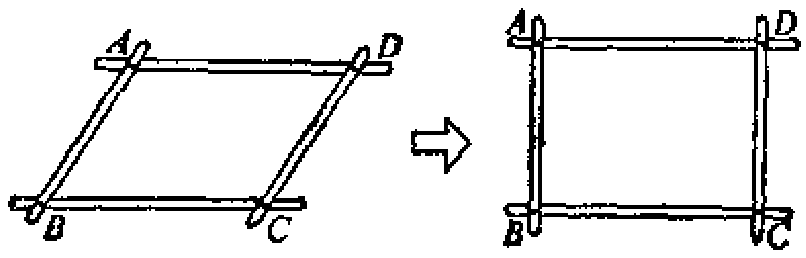
\includegraphics[width=6cm]{../pic/czjh1-ch4-20.png}
        \caption{}\label{fig:czjh1-4-20}
    \end{minipage}
    \qquad
    \begin{minipage}[b]{4cm}
        \centering
        \begin{tikzpicture}
    \tkzDefPoints{0/0/B,  2.5/0/C, 0/1.5/A, 2.5/1.5/D}
    \tkzDrawPolygon(A,B,C,D)
    \tkzMarkRightAngle(D,A,B)
    \tkzMarkRightAngle(A,B,C)
    \tkzMarkRightAngle(B,C,D)
    \tkzMarkRightAngle(C,D,A)
    \tkzLabelPoints[left](A,B)
    \tkzLabelPoints[right](C,D)
\end{tikzpicture}


        \caption{}\label{fig:czjh1-4-21}
    \end{minipage}
    \qquad
    \begin{minipage}[b]{4cm}
        \centering
        \begin{tikzpicture}
    \tkzDefPoints{0/0/B,  2.5/0/C, 0/1.5/A, 2.5/1.5/D}
    \tkzDrawPolygon(A,B,C,D)
    \tkzDrawSegments(A,C  B,D)
    \tkzLabelPoints[left](A,B)
    \tkzLabelPoints[right](C,D)
\end{tikzpicture}


        \caption{}\label{fig:czjh1-4-22}
    \end{minipage}
\end{figure}


\begin{dingli}[矩形性质定理1]
    矩形的四个角都是直角。
\end{dingli}

矩形还有下面的性质:

\begin{dingli}[矩形性质定理2]
    矩形的对角线相等。
\end{dingli}


已知:矩形 $ABCD$ (图 \ref{fig:czjh1-4-22})。

求证:$AC = DB$。

证明: 在矩形 $ABCD$ 中,

$\angle ABC = \angle DCB = Rt \angle$ (矩形的四个角都是直角)。

$AB = DC$(平行四边形的对边相等),

$BC = CB$,

$\therefore$ \quad $\triangle ABC \quandeng \triangle DCB$。

$\therefore$ \quad $AC = DB$。


要判定一个四边形是矩形,除了根据定义判定外,还可以根据下面的定理:

\begin{dingli}[矩形判定定理1]
    有三个角是直角的四边形是矩形。
\end{dingli}


\begin{dingli}[矩形判定定理2]
    对角线相等的平行四边形是矩形。
\end{dingli}


已知: $\pxsbx ABCD$ 中, $AC = DB$(图 \ref{fig:czjh1-4-22})。

求证:$\pxsbx ABCD$ 是矩形。

证明: $\because$ \quad $AC = DB$,$BC = CB$,

\qquad $AB = DC$ (平行四边形的对边相等),

$\therefore$ \quad $\triangle ABC \quandeng \triangle DCB$。

$\therefore$ \quad $\angle ABC = \angle DCB$。

又 $\because$ \quad $AB \pingxing DC$,

$\therefore$ \quad $\angle ABC + \angle DCB = 2 Rt \angle$。

$\therefore$ \quad $\angle ABC = Rt \angle$。

$\therefore$ \quad $\pxsbx ABCD$ 是矩形。

在生产中,工人师傅在制作门框或矩形零件时,常用测量两条对角线是否相等来检查直角的精度,就是根据这个定理。


\begin{enhancedline}
\liti[0] 已知:如图 \ref{fig:czjh1-4-23}, 矩形 $ABCD$ 的两条对角线相交于点 $O$, $\angle AOD = 120^\circ$,
$AB = 4\;\limi$。 求矩形对角线的长。

\begin{wrapfigure}[8]{r}{5cm}
    \centering
    \begin{tikzpicture}
    \tkzDefPoints{0/0/B,  2.5/0/C, 0/1.5/A, 2.5/1.5/D}
    \tkzInterLL(A,C)(B,D)  \tkzGetPoint{O}
    \tkzDrawPolygon(A,B,C,D)
    \tkzDrawSegments(A,C  B,D)
    \tkzLabelPoints[left](A,B)
    \tkzLabelPoints[right](C,D)
    \tkzLabelPoints[above](O)
\end{tikzpicture}


    \caption{}\label{fig:czjh1-4-23}
\end{wrapfigure}


\jie $\because$ \quad 四边形 $ABCD$ 是矩形,

$\therefore$ \quad $AC = BD$ (矩形的对角线相等)。

又 $\because$ \quad \begin{zmtblr}[t]{}
    $OA = OC = \exdfrac{1}{2} AC$, \\[1em]
    $OB = OD = \exdfrac{1}{2} BD$ (平行四边形的对角线互相平分),
\end{zmtblr}

$\therefore$ \quad $OA = OD$。

$\because$ \quad $\angle AOD = 120^\circ$,

$\therefore$ \quad $\angle ODA = \angle OAD = \dfrac{180^\circ - 120^\circ}{2} = 30^\circ$。

又 $\because$ \quad $\angle DAB = Rt \angle$ (矩形的四个角都是直角),

$\therefore$ \quad $BD = 2 AB = 2 \times 4 \;\limi = 8\;\limi$。
\end{enhancedline}


\begin{lianxi}

\xiaoti{求证: 四个角都相等的四边形是矩形。}

\xiaoti{求证: 对角线互相平分并且相等的四边形是矩形。}

\xiaoti{用刻度尺怎样检查一个四边形零件是不是矩形。}

\xiaoti{利用矩形性质, 证明直角三角形斜边上的中线等于斜边的一半。}

\end{lianxi}

